\documentclass{beamer}

% Copyright 2010 Drow Ltd.
% 
% In principle, this file can be redistributed and/or modified under
% the terms of the GNU Public License, version 2.
% 
% However, this file is supposed to be a template to be modified
% for your own needs. For this reason, if you use this file as a
% template and not specifically distribute it as part of a another
% package/program, I grant the extra permission to freely copy and
% modify this file as you see fit and even to delete this copyright
% notice. 
\mode<presentation>
{
  \usetheme[titleline=true,
  alternativetitlepage=true,
  titlepagelogo=images/Java_logo]{Torino}
  \usecolortheme{nouvelle}
  \beamertemplatenavigationsymbolsempty
}

\usepackage{times}
\usepackage[utf8]{inputenc}
\usepackage[english,bulgarian]{babel}
\usepackage[T2A]{fontenc}

\usepackage{listings}
\lstset{language=Java,
  captionpos=b,
  tabsize=4,
  keywordstyle=\color{blue},
  commentstyle=\color{gray},
  stringstyle=\color{green},
  numbers=left,
  breaklines=true,
  showstringspaces=false,
  basicstyle=\ttfamily,
  emph={label},
  frame=shadowbox, 
  rulesepcolor=\color{blue},
  columns=fixed}

\title{Изключения, проверки и журнали в Java. Дебъгване.}

\author{инж. Божидар ~Бацов}

\institute{Drow Ltd.}

\date{21.12.2010}

\subject{Talks}
% This is only inserted into the PDF information catalog. Can be left
% out. 

\begin{document}

\begin{frame}
  \titlepage
\end{frame}

\begin{frame}{Съдържание}
  \transdissolve
  \tableofcontents[pausesections]
\end{frame}

\section{Изключения}

\subsection{Грешки}

\begin{frame}{Грешки в приложенията}
  \transdissolve
  \begin{itemize}
  \item Програмни грешки \pause
    \begin{itemize}
      \item възникват по вина на програмиста \pause
    \end{itemize}
  \item Потребителски грешки \pause
      \begin{itemize}
        \item възникват по вина на потребителя \pause
        \item неподходящи входни данни \pause
        \item неправилна конфигурация \pause
      \end{itemize}
  \item Системни грешки \pause
  \begin{itemize}
    \item липсва на оперативна памет \pause
    \item липса на файлови дескриптори \pause
  \end{itemize}
  \end{itemize}
\end{frame}

\begin{frame}{Класически подход за следене за грешки}
  \transdissolve
  \begin{itemize}
  \item Връщане на специални стойности \pause
    \begin{itemize}
      \item -1 \pause
      \item null \pause
    \end{itemize}
  \item Проблеми на подхода \pause
    \begin{itemize}
      \item върнатите стойности могат лесно да бъдат игнорирани \pause
      \item връщането на null създава риск за възникване на
        NullPointerException \pause
      \item не винаги има подходящи специални стойности
    \end{itemize}

  \end{itemize}
\end{frame}

\begin{frame}{Изключение}
  \transdissolve
  \begin{itemize}
  \item Специален обект, който сигнализира за възникването на някакво
    неочаквано събитие \pause
  \item Капсулира в себе си причина, съобщение за грешка, stack trace \pause
  \item Съществува цяла инфраструктура за обработка на изключения
  \end{itemize}
\end{frame}


\begin{frame}{Йерархия на изключенията}
  \transdissolve
  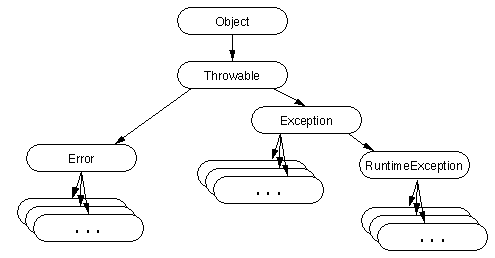
\includegraphics[height=150px,width=300px]{images/throwableHierarchy}
\end{frame}

\begin{frame}{Основни класове в йерархията}
  \transdissolve
  \begin{itemize}
  \item Throwable \pause
    \begin{itemize}
    \item всички изключения го разширяват \pause
    \end{itemize}
  \item Error \pause
    \begin{itemize}
      \item базов клас за изключения свързани с виртуалната машина \pause
      \item не трябва да го разширявате \pause
    \end{itemize}
  \item RuntimeException \pause
    \begin{itemize}
      \item базов клас за изключения свързани с програмни грешки \pause
    \end{itemize}
  \item Exception \pause
    \begin{itemize}
    \item базов клас за всички останали изключения
    \end{itemize}
  \end{itemize}
\end{frame}

\begin{frame}{Видове изключения}
  \transdissolve
  \begin{itemize}
  \item Проверени(checked) \pause
    \begin{itemize}
      \item обработката им се проверява автоматично от компилатора \pause
      \item обекти от подкласове на Exception \pause
      \item Често срещани проверени изключения \pause
        \begin{itemize}
          \item IOException \pause
          \item FileNotFoundException \pause
        \end{itemize}
    \end{itemize}

  \item Непроверени(unchecked) \pause
    \begin{itemize}
      \item възникват от програмни грешки \pause
      \item възникват от грешки във виртуалната машина \pause
      \item обекти от подклас на RuntimeException \pause
      \item Често срещани непроверени изключения
        \begin{itemize}
          \item NullPointerException
          \item InvalidArgumentException
          \item InvalidStateException
          \item OutOfMemoryError
          \item ArithmethicException
        \end{itemize}

    \end{itemize}

  \end{itemize}
\end{frame}

\begin{frame}{Дефиниране на изключения}
  \transdissolve
  \begin{itemize}
  \item Предпочитайте изключенията от стандартната библиотека \pause
  \item Предпочитайте вече дефинирани изключения в рамките на
    приложението ви \pause
  \item Използвайте за базови класове само Exception и
    RuntimeException \pause
  \item В никакъв случай не наследявайте директно Throwable или Error
  \end{itemize}
\end{frame}

\begin{frame}[fragile]
  \frametitle{Пример}
  \transdissolve
\begin{lstlisting}
class MyException extends Exception {
  public MyException() {};

  public MyException(String message) {
    super(message);    
  }
  
  public MyException(String message, Throwable cause) {
    super(message, cause);  
  }
}    
\end{lstlisting}
\end{frame}

\begin{frame}{Работа с изключения}
  \transdissolve
  \begin{itemize}
  \item Изключенията се сигнализират с ключовата дума throw
    \begin{itemize}
      \item \lstinline$throw new SomeException()$ \pause
    \end{itemize}
  \item Изключенията се прихващата в try блок \pause
  \item Изключенията могат да бъдат предадени към извикващия метод
    посредством throws директивата
  \end{itemize}
\end{frame}

\begin{frame}[fragile]
  \frametitle{Пример}
  \transdissolve
\begin{lstlisting}
public void someMethod() throws SomeException {
  try {
    // code that may throw
    // some exception
    ... 
  }
  catch (SomeException e) {
    // handle the exception
    ...
  } finally {
    // do some cleanup
    ...
  }
}
  
\end{lstlisting}
\end{frame}

\begin{frame}{Работа с изключения}
  \transdissolve
  \begin{itemize}
  \item Има смисъл да се прихващат само изключения, за които може да
    бъде направено нещо \pause
  \item Има смисъл да се пропагират(предават нагоре) само проверени изключения \pause
  \item Код във finally блок се изпълнява винаги 
  \end{itemize}
\end{frame}

\begin{frame}{Stack trace}
  \transdissolve
  \begin{itemize}
  \item Информация за реда на извиквания на методи  \pause
  \item Съдържа се във всяко изключение \pause
  \item Изключително полезен при дебъгване за определяне на мястото,
    на което е възникнал даден проблем
  \end{itemize}
\end{frame}

\begin{frame}{Опаковане на изключения}
  \transdissolve
  \begin{itemize}
  \item Едно изключение може да е причинено от друго \pause
  \item Причината(cause) се задава в конструктора на новото изключение \pause
  \item Често се използва за опакова на проверени изключения в непроверени
  \end{itemize}
\end{frame}

\begin{frame}{Добри практики}
  \transdissolve
  \begin{itemize}
  \item Предпочитай стандартните изключения \pause
  \item Използвайте ги само, когато наистина се нуждаете от тях \pause
  \item Не ги потискайте \pause
  \item Избягвайте прекалената употреба на проверени изключения
  \end{itemize}
\end{frame}

\section{Проверки}

\begin{frame}{Проверки(Assertions)}
  \transdissolve
  \begin{itemize}
  \item Използват се за потвърждаване на коректността на стойности в
    определени моменти от програмата \pause
  \item Извършват се с ключовата дума assert \pause
  \item Проверките се активират на ниво виртуална машина с флага -еа
  \end{itemize}
\end{frame}

\begin{frame}{Работа с проверки}
  \transdissolve
  \begin{itemize}
  \item При пропадане на проверка програмата завършва с AssertionError \pause
  \item Използват се само във фазата на разработка \pause
  \item В режим на експлоатация(production deployment) се изключват на
    ниво виртуална машина \pause
  \item Употреба
    \begin{itemize}
      \item \lstinline$assert condition$;
      \item \lstinline$assert condition : expression$;
    \end{itemize}
  \end{itemize}
\end{frame}

\begin{frame}[fragile]
  \frametitle{Пример}
  \transdissolve
\begin{lstlisting}
assert true;
assert 5 > 4;
assert someList.isEmpty();
assert someList.size() > 10 : "Big trouble";
\end{lstlisting}
\end{frame}


\section{Журнали}

\begin{frame}{Програмен журнал}
\transdissolve
\begin{itemize}
\item Информативни съобщения, чрез които можем да анализираме работата
  на дадено приложение \pause
\item Категории журнални съобщения
\begin{itemize}
  \item debug
  \item info
  \item warning
  \item error \pause
\end{itemize}
\item Извеждане на конзола \pause
\item Съхранение във файл \pause
\begin{itemize}
  \item ротация на журналните съобщения
\end{itemize}
\end{itemize}
\end{frame}

\begin{frame}{Журналния библиотеки в Java}
  \transdissolve
  \begin{itemize}
  \item Java Logging \pause
  \item Log4J \pause
  \item Logback \pause
  \item SimpleLog \pause
  \item Фасадни библиотеки
    \item Commons Logging
    \item SLF4J
  \end{itemize}
\end{frame}

\begin{frame}{Работа с журнални библиотеки}
  \transdissolve
  \begin{itemize}
  \item Обикновено се конфигурират с конфигурационен файл или
    програматично \pause
  \item Стандартни опции
    \begin{itemize}
      \item описателност(verbosity)
      \item дестинация(конзола, файл)
      \item формат на съобщенията
      \item ротация/архивиране
    \end{itemize}
  \end{itemize}
\end{frame}

\begin{frame}{Добри практики при водене на журнал}
  \transdissolve
  \begin{itemize}
  \item Всеки клас, който прави нещо смислено трябва да има
    Logger(private static final) \pause
  \item Журналните съобщения не трябва да са криптични, а ясни и
    описателни \pause
  \item Дръжте конфигурацията си в конфигурационни файлове, а не в
    кода \pause
  \item Предпочитайте фасадни библиотеки
  \end{itemize}
\end{frame}


\section{Дебъгване}

\begin{frame}{Дебъгване тип "`старата школа"}
  \transdissolve
  \begin{itemize}
  \item println до дупка
  \end{itemize}
\end{frame}

\begin{frame}{Дебъгване с дебъгер}
  \transdissolve
  \begin{itemize}
  \item Най-мощната техника за търсене и отстраняване на проблеми \pause
  \item Дебъгерът ви дава възможност да:
    \begin{itemize}
      \item спрете изпълнение на програмата в даден момент \pause
      \item прегледате стойностите на полета, локални променливи \pause
      \item да изпълнявате програмата твърдение по твърдение \pause
      \item да изпълнявате произволни твърдения в контекста на
        текущата програма 
    \end{itemize}

  \end{itemize}
\end{frame}

\begin{frame}{Работа с дебъгер}
  \transdissolve
  \begin{itemize}
  \item Интегриран в повечето среди за разработка \pause
  \item Поставяне на точки на прекъсване(line break, method break,
    etc) \pause
  \item Стартиране на приложението в debug режим \pause
  \item Програмата спира(прави пауза) на първата срещната точка за
    прекъсване
  \end{itemize}
\end{frame}

\begin{frame}{Добри практики при работа с дебъгер}
  \transdissolve
  \begin{itemize}
  \item Използвайте stack trace-a, за да определените местата за точки
    на прекъсване \pause
  \item Развийте навик да преглеждате състоянието на всички по-важни
    стойности \pause
  \item Избягвайте употребата на method точки за прекъсване
  \end{itemize}
\end{frame}


\section*{Заключение}

\begin{frame}{Заключение}
  \transdissolve
  % Keep the summary *very short*.
  \begin{itemize}
  \item
    Ползвайте изключения за обработка на изключителни събития.
  \item
    Използването на проверки и журнал води до по-устойчив на грешки софтуер.
  \item
    Грешките са част от програмирането и в борбата с тях дебъгерът е
    най-добрият ви приятел.
  \end{itemize}
  
  % The following outlook is optional.
  \vskip0pt plus.5fill
  \begin{itemize}
  \item
    Следващият път:
    \begin{itemize}
    \item Генерично програмиране
    \end{itemize}
  \end{itemize}
\end{frame}

\begin{frame}{Въпроси}
  \transdissolve
  \begin{center}
    \LARGEТук е момента да зададете вашите въпроси! :-)
  \end{center}
\end{frame}

\begin{frame}{Край}
  \transdissolve
  \begin{center}
    \LARGEБлагодаря Ви за вниманието!
  \end{center}
\end{frame}

\end{document}

%%% Local Variables: 
%%% mode: latex
%%% TeX-master: t
%%% End: 
